\documentclass[a4paper, 11pt]{article}
\usepackage[utf8]{inputenc}
\usepackage[T1]{fontenc}
\usepackage[top=3cm, text={17cm, 24cm}, left=2cm]{geometry}
\usepackage[czech]{babel}
\usepackage{booktabs}
\usepackage{graphicx}
\usepackage{float}

\begin{document}

\begin{titlepage}
\begin{center}
    \Huge
    \textsc{Vysoké učení technické v~Brně\\
    \huge{Fakulta informačních technologií}}\\
    \vspace{\stretch{0.382}}
    \LARGE{Zpracování a vizualizace dat v~prostředí Python}\\
    \Huge{Analýza nehod s~chodcem na základě reflexních prvků}\\
    \vspace{\stretch{0.618}}
\end{center}
{\Large \today \hfill Michal Blažek}
\end{titlepage}

\section{Příprava dat}

Pro zkoumání efektivity reflexních prvků na chodcích jsou potřeba data z~nehod a konkrétně informace srážek s~chodcem (sloupec p6 a jeho hodnota 4), zda chodec na sobě měl reflexní prvky (sloupec p29a), jaká byla viditelnost (sloupec p19) a následky na zdraví chodců (sloupec p33g). Tato analýza je zaměřena na sníženou viditelnost, která má v~připravených datech jakoukoliv hodnotu větší jak 1, jelikož hodnota 1 značí nezhoršenou viditelnost vlivem povětrnostních podmínek ve dne.

\section{Vlastní analýza a výsledky}

Připravená data mají 2 veličiny, a to je přítomnost reflexních prvků u~chodce a následky na zdraví chodce. Pomocí těchto 2 veličin se vytvoří kontingenční tabulka, která se nachází v~tabulce \ref{tab:reflexni_prvky}.

\begin{table}[H]
    \centering
    \begin{tabular}{|l|c|c|c|c|}
        \toprule
        Zranění & Bez zranění & Lehké zranění & Těžké zranění & Usmrcení \\
        Přítomnost reflexních prvků &  &  &  &  \\
        \midrule
        \textbf{Ano} & 3 & 57 & 8 & 1 \\
        \textbf{Ne} & 148 & 1033 & 176 & 59 \\
        \bottomrule
    \end{tabular}
    \caption{Kontingenční tabulka následků nehody s~chodcem s~reflexními prvky a bez nich.}
    \label{tab:reflexni_prvky}
\end{table}

Pomocí sloupcového grafu na obrázku \ref{fig:pocet_nehod} lze vidět značně zvýšený počet nehod s~chodci bez reflexních prvků. Po sečtení všech hodnot v~jednotlivých sloupcích dostaneme počet všech zranění.

\begin{eqnarray}
    \label{eq:pocet_s_reflex}57+8+3+1 & = & 69\\
    \label{eq:pocet_bez_reflex}1033+176+148+59 & = & 1416\\
    \label{eq:nasobek_nehod_bez_reflex}1416\div 69 & \approx & 20,52
\end{eqnarray}

Ve výsledku výpočtu \ref{eq:pocet_s_reflex} lze vidět 69 nehod celkem s~chodci, které nosili reflexní prvky, zatímco s~těmi, co na sobě neměli reflexní prvky, je počet nehod z~výpočtu \ref{eq:nasobek_nehod_bez_reflex} více než 20krát větší. Celkový počet nehod s~chodci bez reflexních prvků se nachází ve výpočtu \ref{eq:pocet_bez_reflex}, a to je 1416 nehod.

Samotná závažnost zranění se ovšem moc neliší u~chodců s~reflexními prvky a u~chodců bez nich, což je vidět na výpočtech \ref{eq:zavaznost_zraneni_s_reflex} pro chodce s~reflexními prvky a \ref{eq:zavaznost_zraneni_bez_reflex} pro chodce bez nich. Pravděpodobně to bude způsobeno nepozorností řidičů. Pokud řidič přehlédne chodce i s~reflexními prvky nebo se stane jiná nečekaná situace, pravděpodobně způsobená zranění u~chodců nejsou o~nic lehčí. Tyto výpočty předpokládají hodnoty jednotlivých zranění z~tabulky \ref{tab:zraneni_hodnota}, a tudíž vypočítané hodnoty značí průměrně lehké zranění u~chodců.

\begin{eqnarray}
    \label{eq:zavaznost_zraneni_s_reflex}\frac{3\times0+57\times1+8\times2+1\times3}{69} & \approx & 1,1014\\[12pt]
    \label{eq:zavaznost_zraneni_bez_reflex}\frac{148\times0+1033\times1+176\times2+59\times3}{1416} & \approx & 1,1031
\end{eqnarray}

Lze tedy z~analýzy a jejich výsledků určitě doporučit nosit reflexní prvky za snížené viditelnosti, ale i za nesnížené, jelikož díky reflexním prvkům je chodec více vidět a řidiči jej mohou spatřit i na větší vzdálenost. Ovšem i chodem musí být na pozoru, protože reflexní prvky mu nezmírní závažnost potencionálního zranění.

\begin{table}[H]
    \centering
    \begin{tabular}{|l|c|}
        \toprule
        Závažnost zranění & Hodnota zranění \\
        \midrule
        Bez zranění & 0 \\
        Lehké zranění & 1 \\
        Těžké zranění & 2 \\
        Usmrcení & 3 \\
        \bottomrule
    \end{tabular}
    \caption{Tabulka hodnot zranění podle závažnosti.}
    \label{tab:zraneni_hodnota}
\end{table}

\begin{figure}[H]
    \centering
    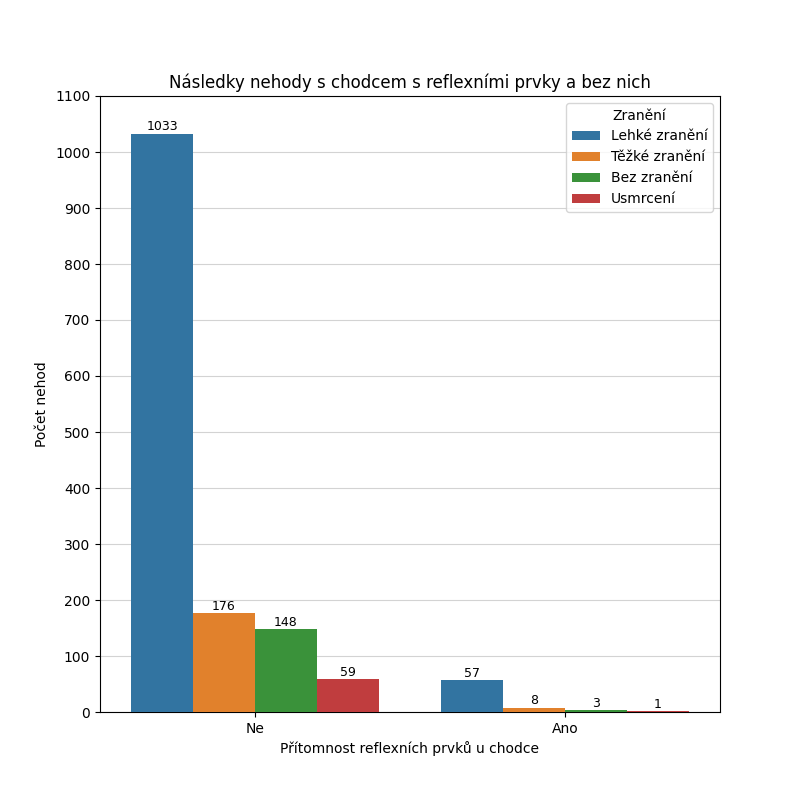
\includegraphics[width=1.0\textwidth]{fig.png}
    \caption{Graf znázorňuje počet nehod s~chodcem za snížené viditelnosti s~reflexními prvky chodce a bez nich. Jednotlivé sloupce značí závažnost zranění, které chodem z~nehody má.}
    \label{fig:pocet_nehod}
\end{figure}

\end{document}
